\subsection{Operacje na mapach bitowych}
\label{subsec:operacje-na-mapach-bitowych}

Jak już wcześniej wspomniano, iteracyjne generowanie ruchów każdej z bierek z osobna mogłoby okazać się zbyt czasochłonne.
Z tego względu większość dostępnych posunięć tworzona jest dzięki przekształcaniu map bitowych reprezentujących konkretny typ figury.
Optymalizacja przynosi szczególny efekt przy generowaniu ruchów pionów, ze względu na~ich~znaczną ilość przez większość czasu gry.

Pion ma do dyspozycji kilka możliwych ruchów, które należało zaimplementować: ruch o~jedno pole do przodu, ruch o dwa pola do przodu, bicie w lewo i bicie w prawo.

Maski dla każdego z tych ruchów zostały wygenerowane w oddzielnych metodach.
Przykładowo, dla ruchu o dwa pola do przodu wzór wygląda następująco:
\begin{align*}
    moves & = empty && \text{pole docelowe musi być puste} \\
    moves & = moves \wedge (pionki_w\ll16) && \text{biały pion musi być dwa wiersze niżej}\\
    moves & = moves \wedge (empty\ll8) && \text{wiersz niżej musi być pusty}\\
    moves & = moves \wedge rank4 && \text{pole docelowe musi być w czwartym wierszu}
\end{align*}

W taki sposób stworzono maskę bitową końcowych pól, na które piony mogą się przesuwać, skacząc o dwa pola.
Na otrzymanym wyniku należy przeprowadzić serializację, to jest przekształcić go na listę dostępnych ruchów.
Aby nie iterować przez wszystkie 64 bity, zastosowano technikę zwaną ang. \emph{Bit Scan}, która zwraca indeks najbardziej istotnego bitu na masce, dodaje ruch do listy, a następnie usuwa ten bit z maski.
Operacja jest wykonywana do~momentu, aż maska pozostanie pusta.
\begin{lstlisting}[
    language=Java,
    style=JavaStyle,
    caption=Metoda dodająca ruchy z maski wraz z przykładowym wywołaniem,
    label=lst:mask]
     addMovesFromMask(movesMask, moveType, offset) {
        while(movesMask != 0L) {
            index = (64 - Long.numberOfLeadingZeros(movesMask));
            possibleMoves.add(new Move(index+offset, index, moveType));
            movesMask &= ~(1L << (index - 1));
        }
     }

    addMovesFromMask(allDoublePushMask, DOUBLE_PAWN_PUSH, -16);

\end{lstlisting}

Legalne ruchy króla i skoczka generowane są w sposób analogiczny, z tą jednak różnicą, że maski dostępnych ruchów tworzone są nie przez przesunięcia bitowe, ale przy inicjalizacji silnika generowana jest tablica dla każdego z pól startowych.

%
%\subsubsection{Generowanie ruchów hetmana, wieży i gońca}
%
%Ruchy hetmana są połączeniem ruchów wieży oraz gońca, z tego względu można je generować w ten sam sposób.
%Techniki te operują na bardzo podobnych zasadach, co generowanie ruchów piona, z tą różnicą, że figury mogą poruszać się o dowolną liczbę pól w danym kierunku, aż do momentu napotkania innej bierki na swojej drodze.
%Aby uniknąć skomplikowanych obliczeń, należało zaimplementować funkcję, która w literaturze znana jest pod nazwą (ang.~\emph{Hyperbola Quintessence}).
%
%\subsubsection{Generowanie ruchów króla i skoczka}


%\begin{figure}[ht]
%    \centering
%    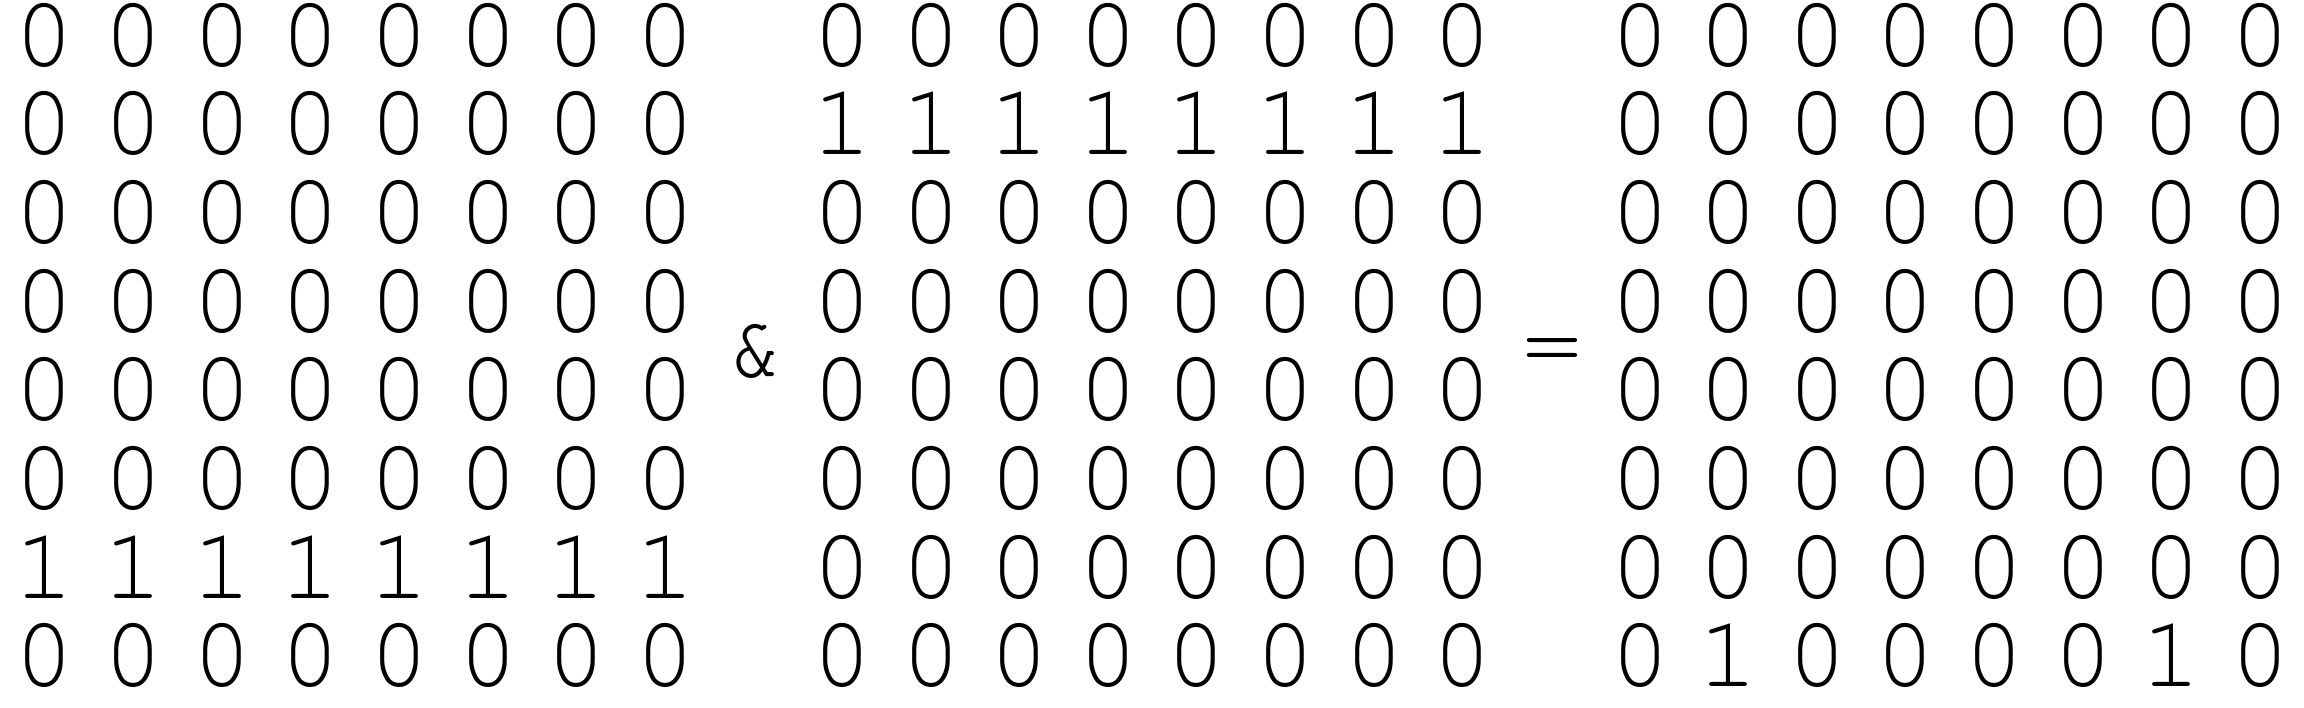
\includegraphics[width=0.85\linewidth]{rozdzialy/rozdzial01/3_generowanie-ruchow/rysunki/bitboards-arithmetic}
%    \caption{Kodowanie ruchu szachowego}
%    \label{fig:bitboards-arithmetic}
%\end{figure}